\clearpage


\section{Campus}

\subsection{Dein Campus}
Der Campus Sankt Augustin, 1995 aufgebaut, ist das Herzstück deines Studiums an der Hochschule Bonn-Rhein-Sieg.  
Hier wirst du die meiste Zeit verbringen, in Vorlesungen, Übungen, beim Lernen in der Bibliothek, in der Mensa, beim Austausch mit deinen Kommillitonen oder einfach bei uns im Büro.  

\subsection{Besonderes Satellitenbild vom Campus}

Normalerweise sind Satellitenbilder in Karten-Apps (Google Maps(unscharf), Apple Maps(alt) usw.) gerade rund um unseren Campus. 
Für dieses Heft hatte ich allerdings Glück: ich konnte ein aktuelles und hochauflösendes Satellitenbild bekommen, das deutlich neuer ist als die gängigen Online-Karten oder zumindest hochauflösend.  

Damit hast du einen der seltenen Blicke auf den Campus „von oben“ in fast aktuellem Zustand. (~Nagut, Timo hier, 10 Monate später. Der Vorhof, Innenhof und Zwischenhof sind nun fertig. Damit ist dieses Bild auch nicht mehr aktuell!
Also, um sich schon einmal zu orientieren und als kleines Extra für dich als Erstsemester, sollte es trotzdem reichen!~) In der PDF kann man recht nah ranzoomen. 



\subsection{Anreise}

Wenn du zu uns an den Campus kommen willst, hast du wirklich alle Optionen.  
Mit dem Auto erreichst du die Hochschule über gleich drei Autobahnabfahrten nach Sankt Augustin oder bequem über die Bundesstraße. Natürlich kannst du auch mit dem Fahrrad kommen, wir hätten sonst auch nicht so viele Möglichkeiten diese zu parken. 

Auch mit dem Bus bist du fast direkt vor der Tür: Die Linie \textbf{540} fährt von Bonn bis zur \textbf{Grantham-Allee}. Von dort sind es nur etwa drei Minuten zu Fuß, einfach die Straße geradeaus hinunter.  

Die meisten kommen jedoch mit der Bahn: Mit der \textbf{Linie 66} aus Siegburg oder Bonn fährst du bis zur Haltestelle \textbf{Sankt Augustin Zentrum}. Von dort sind es etwa zehn Minuten Fußweg zum Campus. Du gehst ggf. über die Gleiswechselbrücke, den \textbf{Huma} (rechts von dir), dann links am Schulkomplex vorbei, anschließend rechts die Treppe hinunter zum \textbf{Technischen Rathaus}. Dort hältst du dich links, gehst an der Turnhalle vorbei, quer über die Parkplätze und schon steht das Hochschulgebäude direkt vor dir.  



\begin{figure}[H]
    \centering
    \includegraphics[width=0.95\textwidth]{./2.0.0.0_content/photos/campus/Satelietenbild.png}
    \label{Satellitenbild unseres Campus (Stand: 0124)}
\end{figure}


\subsection{Lageplan}

\noindent
Dieser Lageplan wurde vom Ersti-Heft-Team erstellt. Wir verteilen die \textbf{SVG} gerne. Wenn du beim Lesen dieses Hefts noch nicht am \textbf{Campus} warst, kannst du dir hier schon einen ersten Überblick verschaffen. Besonders praktisch: Auf dem Plan erkennst du auch einige Details, die man leicht übersieht. Dazu gehören die alten \textbf{Fahrradstellplätze} ganz links außen am Ende von \textbf{Gebäude A5}, die vor einigen Jahren modernisierten Stellplätze zwischen den \textbf{Gebäuden C1 und C2} sowie die neu gebauten, überdachten \textbf{Fahrradstellplätze mit eigenen Garagen}. Ebenfalls eingezeichnet sind die \textbf{Motorradparkplätze} zwischen \textbf{C1 und C2} und die \textbf{E-Ladesäulen} mit den dazugehörigen \textbf{Parkplätzen}, die direkt neben den \textbf{Fahrrad- und Motorradstellplätzen} zu finden sind. Außerdem siehst du die beiden neuen \textbf{Schranken}, die den Zugang zu den \textbf{Parkplätzen P1, P2 und P4} regeln. So bist du bestens vorbereitet, wenn du dich das erste Mal auf dem \textbf{Campus} orientieren musst.

\begin{figure}[H]
    \centering
    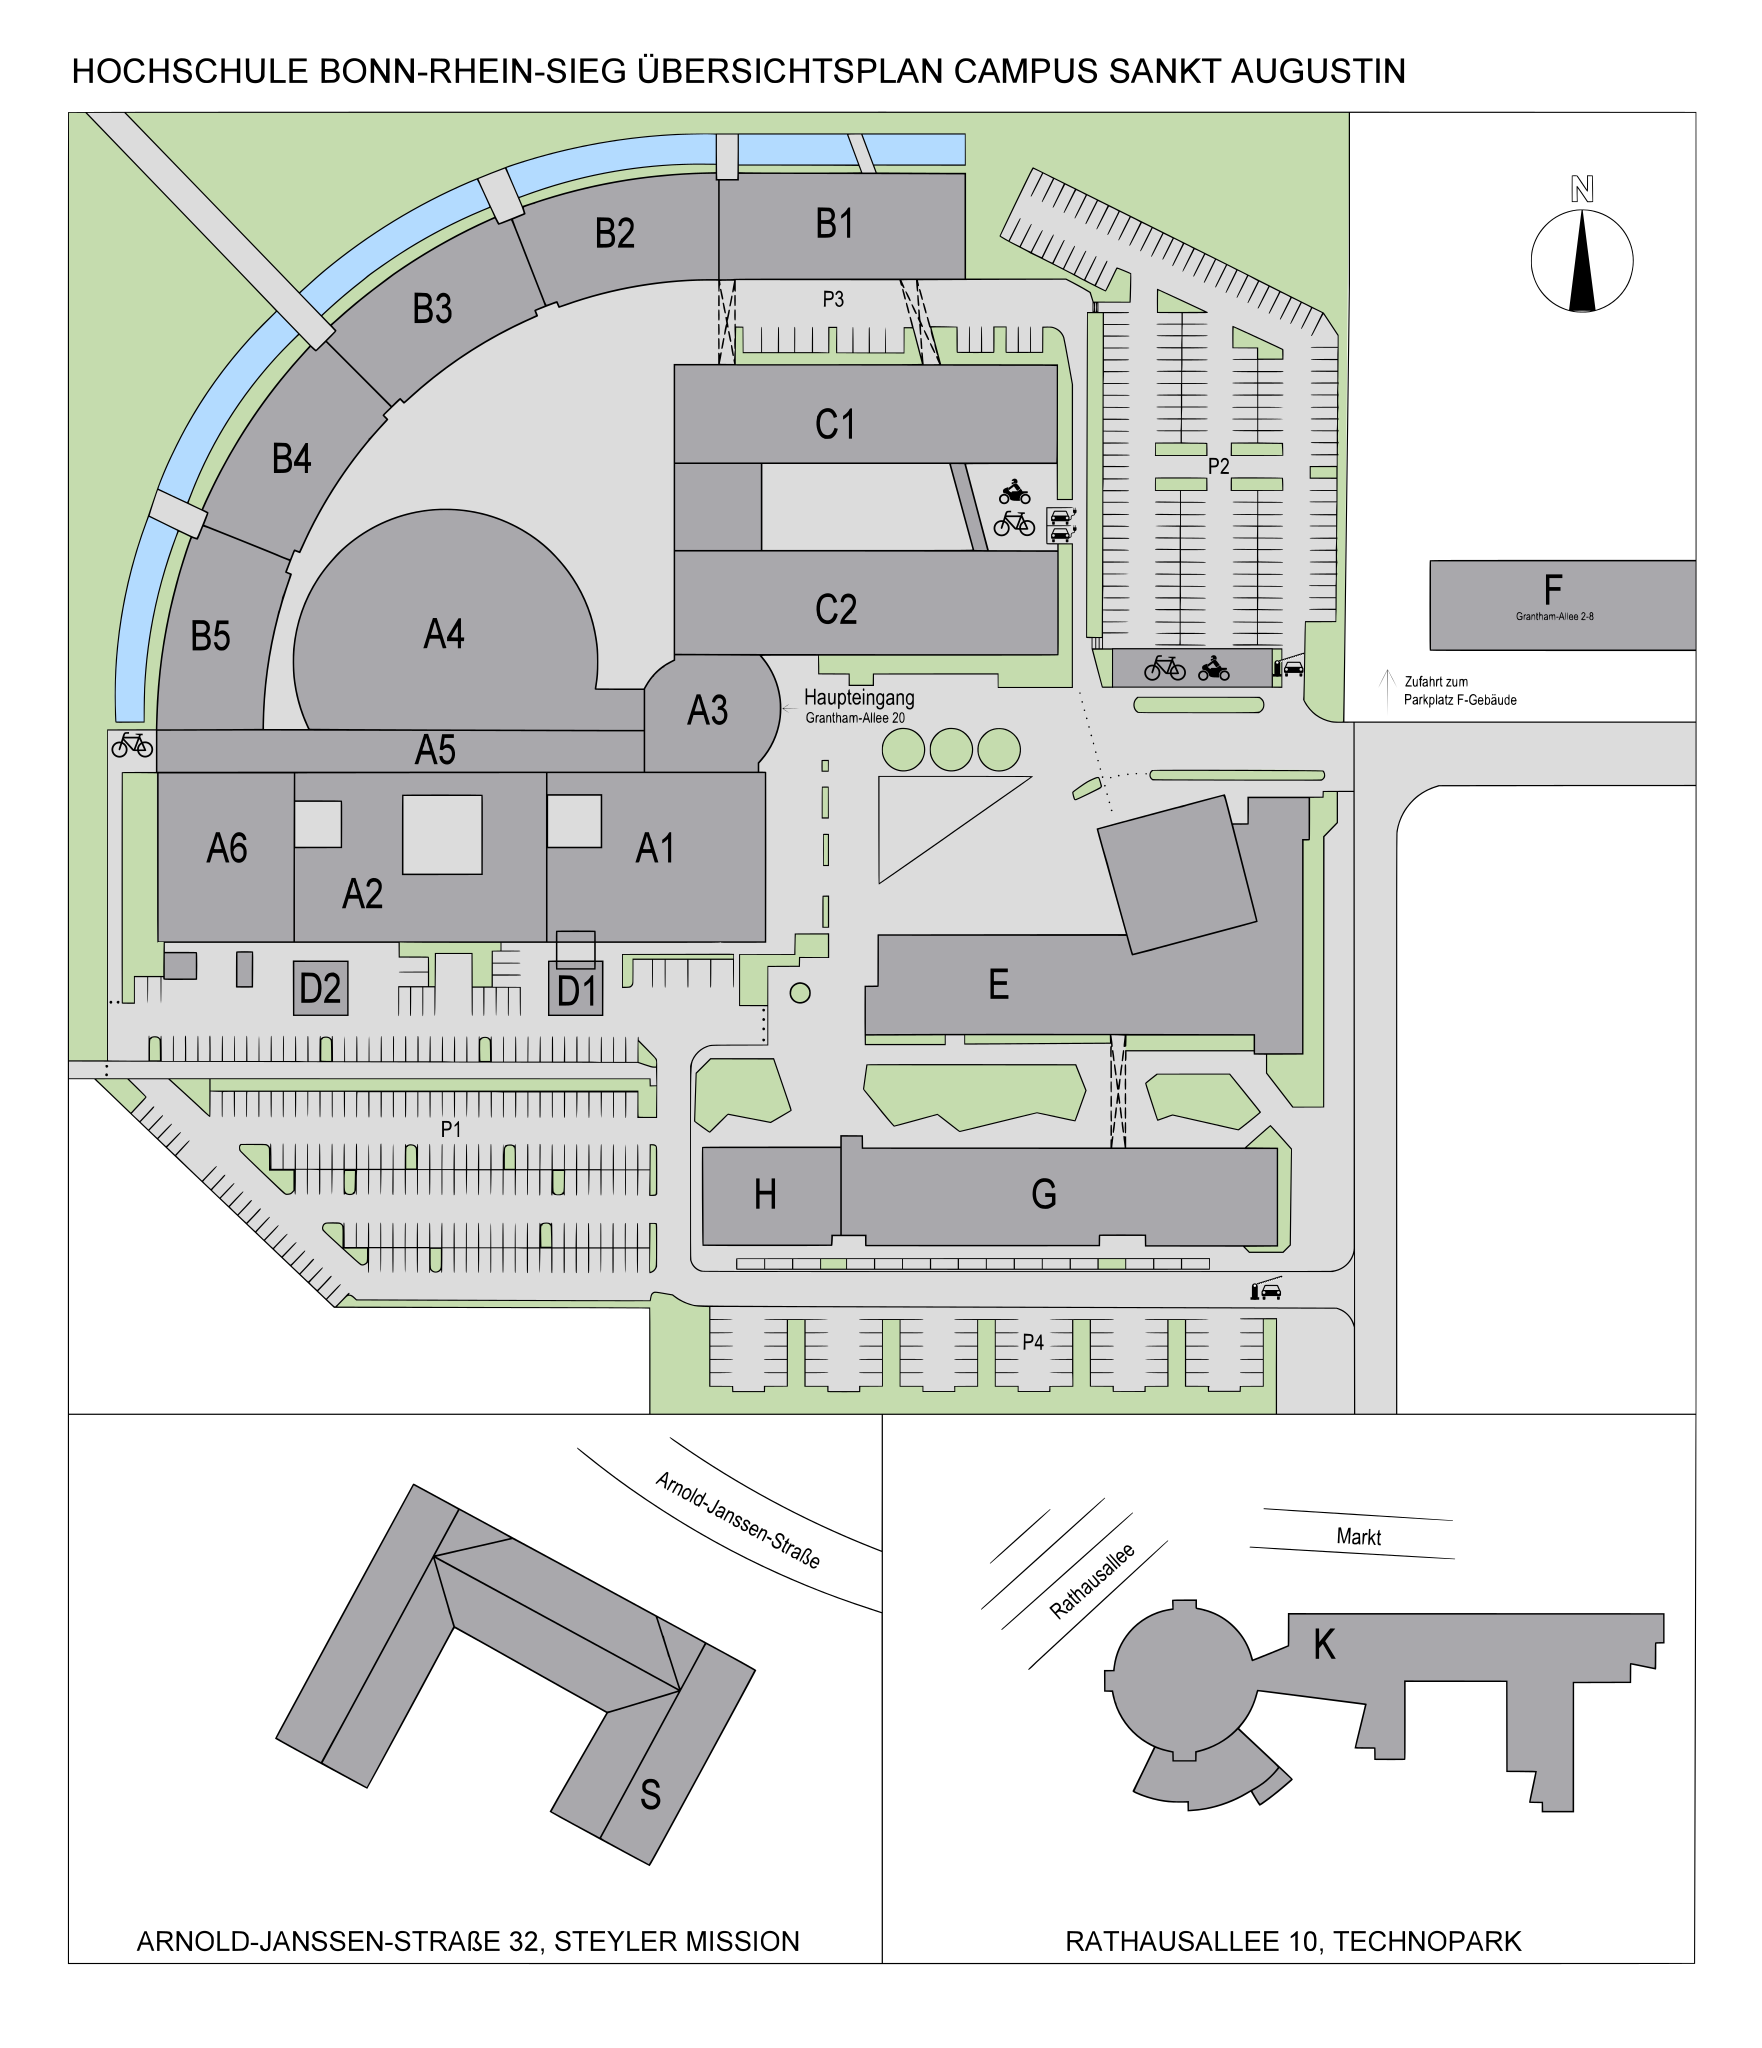
\includegraphics[width=0.95\textwidth]{./2.0.0.0_content/photos/campus/Lageplan-Campus-Sankt-Augustin-2025.png}
    \label{Dieser Lageplan fast aktuell.}
\end{figure}




\clearpage







